% Options for packages loaded elsewhere
\PassOptionsToPackage{unicode}{hyperref}
\PassOptionsToPackage{hyphens}{url}
%
\documentclass[
]{book}
\usepackage{lmodern}
\usepackage{amssymb,amsmath}
\usepackage{ifxetex,ifluatex}
\ifnum 0\ifxetex 1\fi\ifluatex 1\fi=0 % if pdftex
  \usepackage[T1]{fontenc}
  \usepackage[utf8]{inputenc}
  \usepackage{textcomp} % provide euro and other symbols
\else % if luatex or xetex
  \usepackage{unicode-math}
  \defaultfontfeatures{Scale=MatchLowercase}
  \defaultfontfeatures[\rmfamily]{Ligatures=TeX,Scale=1}
\fi
% Use upquote if available, for straight quotes in verbatim environments
\IfFileExists{upquote.sty}{\usepackage{upquote}}{}
\IfFileExists{microtype.sty}{% use microtype if available
  \usepackage[]{microtype}
  \UseMicrotypeSet[protrusion]{basicmath} % disable protrusion for tt fonts
}{}
\makeatletter
\@ifundefined{KOMAClassName}{% if non-KOMA class
  \IfFileExists{parskip.sty}{%
    \usepackage{parskip}
  }{% else
    \setlength{\parindent}{0pt}
    \setlength{\parskip}{6pt plus 2pt minus 1pt}}
}{% if KOMA class
  \KOMAoptions{parskip=half}}
\makeatother
\usepackage{xcolor}
\IfFileExists{xurl.sty}{\usepackage{xurl}}{} % add URL line breaks if available
\IfFileExists{bookmark.sty}{\usepackage{bookmark}}{\usepackage{hyperref}}
\hypersetup{
  pdftitle={URSSI Implementation Plan},
  pdfauthor={Karthik Ram; Jeffrey Carver; Sandra Gesing; Daniel S. Katz; Nic Weber},
  hidelinks,
  pdfcreator={LaTeX via pandoc}}
\urlstyle{same} % disable monospaced font for URLs
\usepackage{longtable,booktabs}
% Correct order of tables after \paragraph or \subparagraph
\usepackage{etoolbox}
\makeatletter
\patchcmd\longtable{\par}{\if@noskipsec\mbox{}\fi\par}{}{}
\makeatother
% Allow footnotes in longtable head/foot
\IfFileExists{footnotehyper.sty}{\usepackage{footnotehyper}}{\usepackage{footnote}}
\makesavenoteenv{longtable}
\usepackage{graphicx}
\makeatletter
\def\maxwidth{\ifdim\Gin@nat@width>\linewidth\linewidth\else\Gin@nat@width\fi}
\def\maxheight{\ifdim\Gin@nat@height>\textheight\textheight\else\Gin@nat@height\fi}
\makeatother
% Scale images if necessary, so that they will not overflow the page
% margins by default, and it is still possible to overwrite the defaults
% using explicit options in \includegraphics[width, height, ...]{}
\setkeys{Gin}{width=\maxwidth,height=\maxheight,keepaspectratio}
% Set default figure placement to htbp
\makeatletter
\def\fps@figure{htbp}
\makeatother
\setlength{\emergencystretch}{3em} % prevent overfull lines
\providecommand{\tightlist}{%
  \setlength{\itemsep}{0pt}\setlength{\parskip}{0pt}}
\setcounter{secnumdepth}{5}
\usepackage{booktabs}
\usepackage{amsthm}
\makeatletter
\def\thm@space@setup{%
  \thm@preskip=8pt plus 2pt minus 4pt
  \thm@postskip=\thm@preskip
}
\makeatother
\usepackage[]{natbib}
\bibliographystyle{apalike}

\title{URSSI Implementation Plan}
\author{Karthik Ram \and Jeffrey Carver \and Sandra Gesing \and Daniel S. Katz \and Nic Weber}
\date{2020-04-10}

\begin{document}
\maketitle

{
\setcounter{tocdepth}{1}
\tableofcontents
}
\hypertarget{welcome}{%
\chapter*{Welcome}\label{welcome}}
\addcontentsline{toc}{chapter}{Welcome}

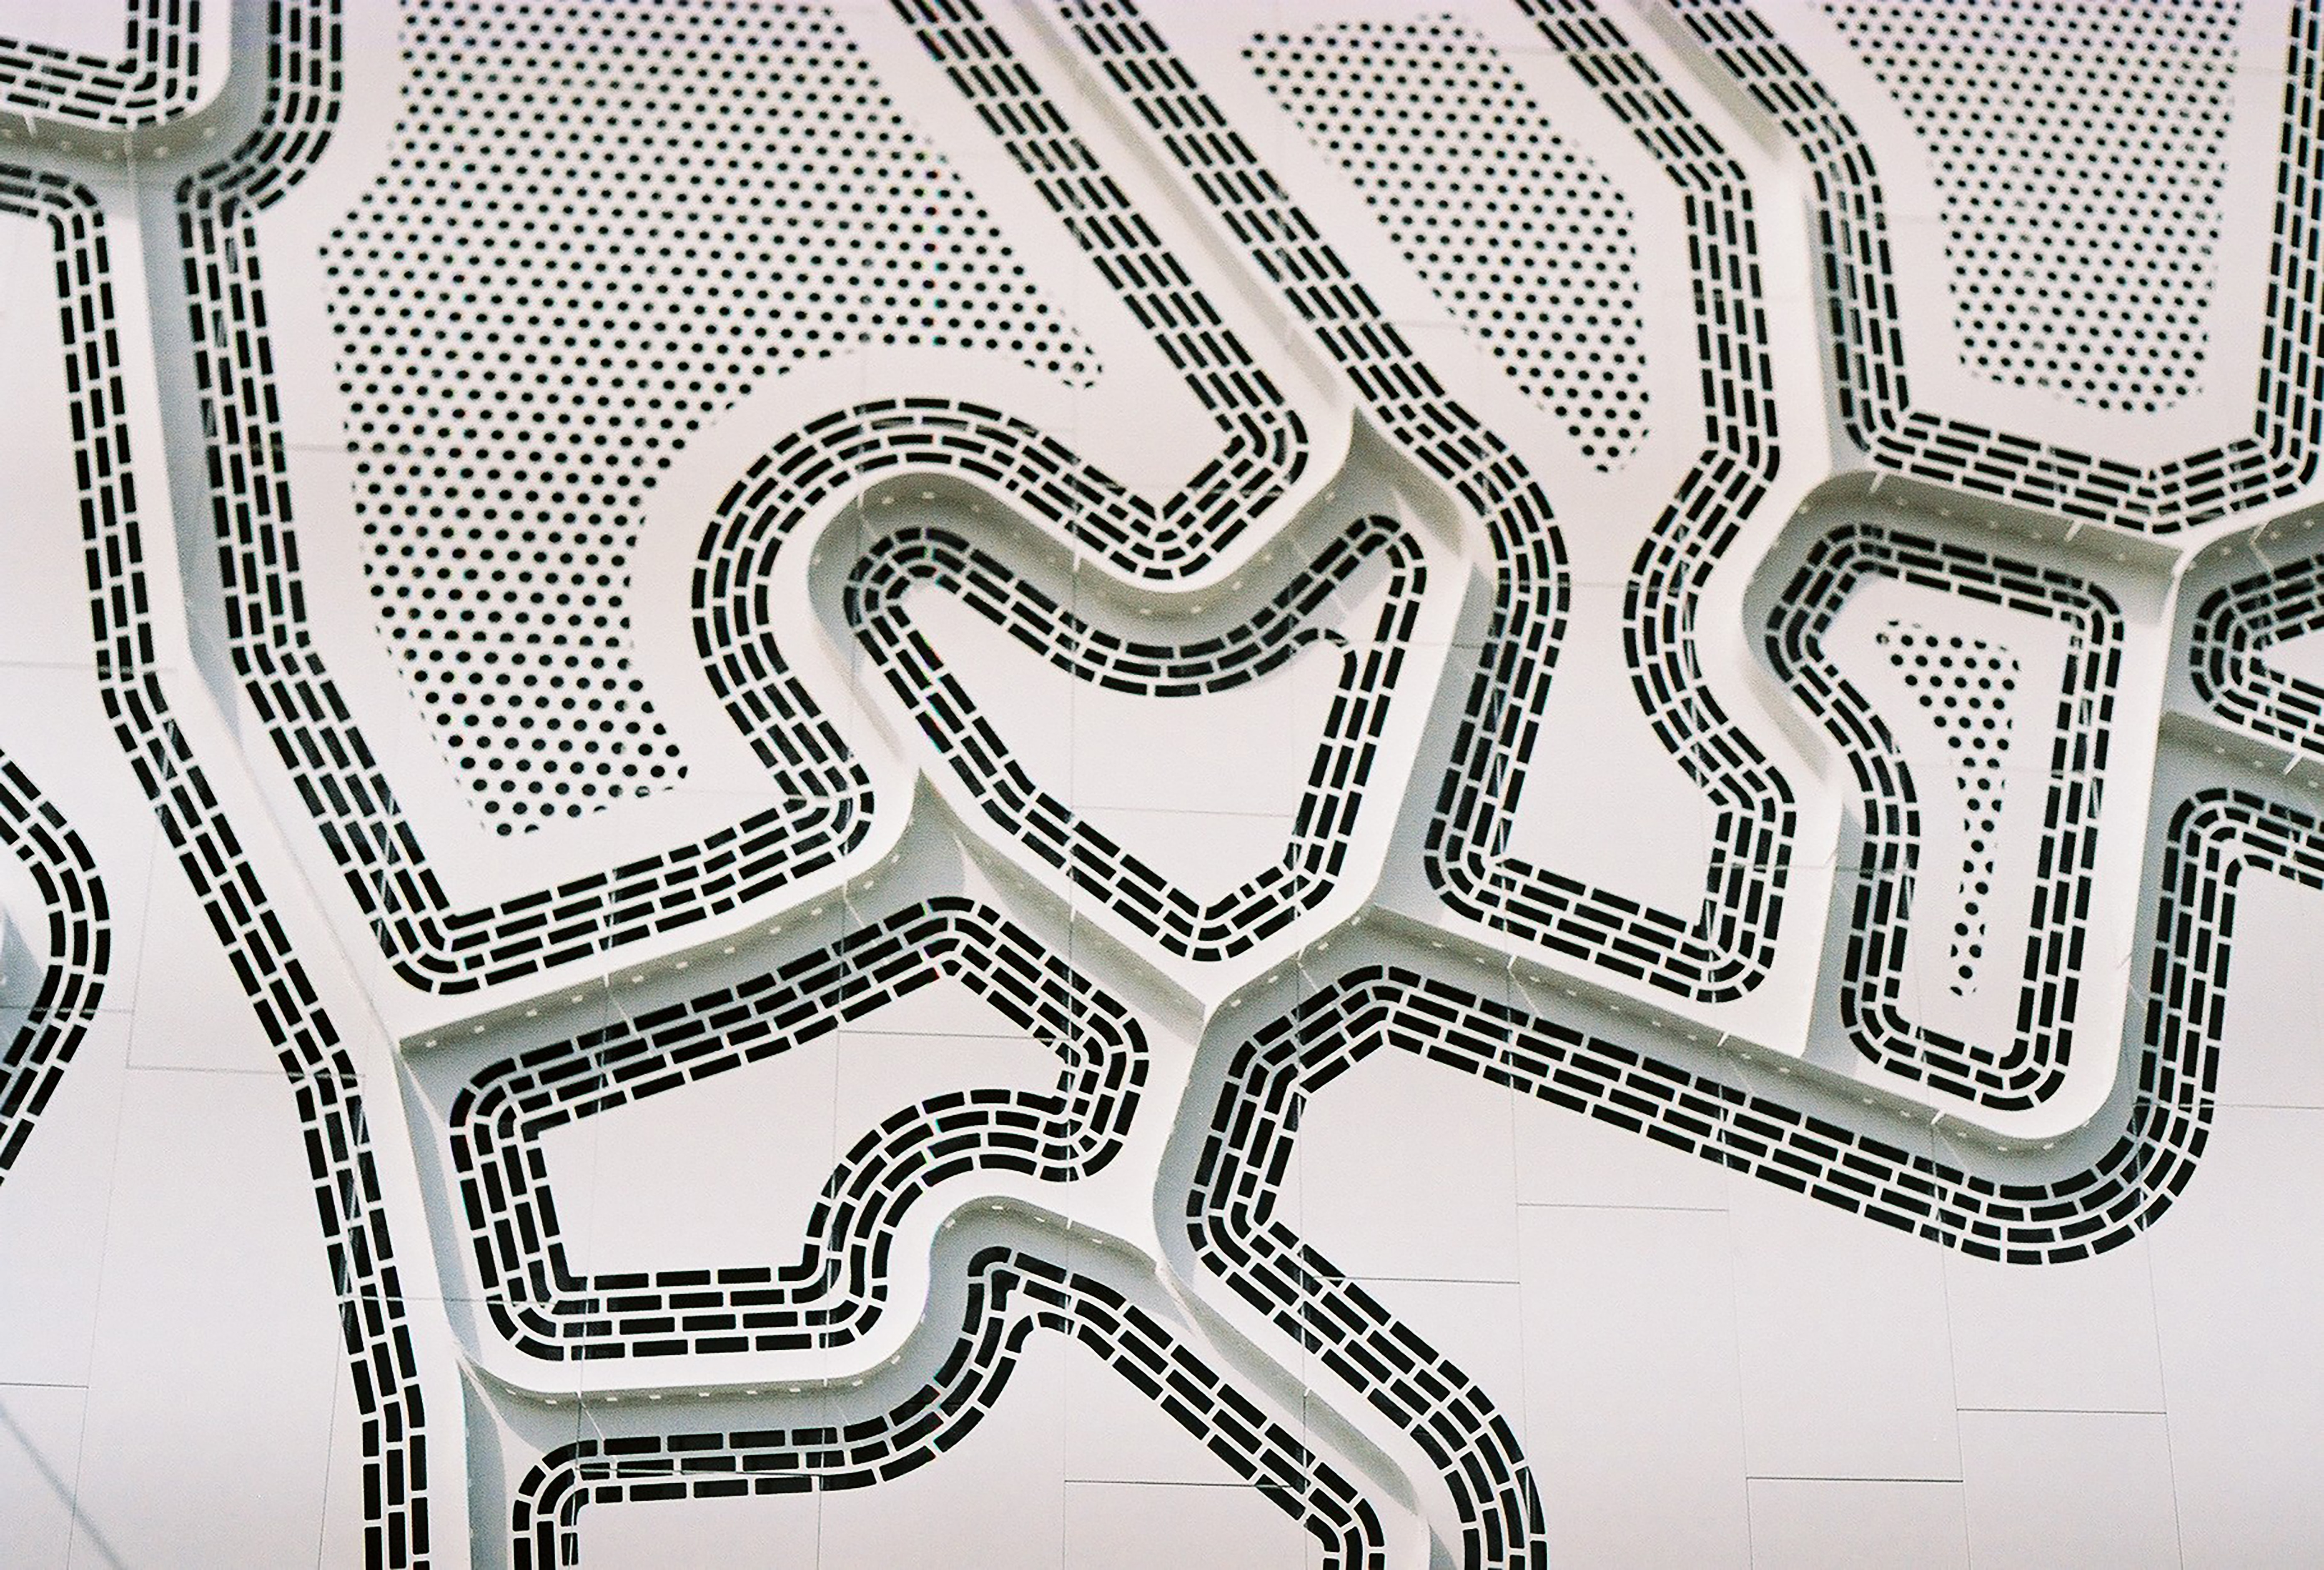
\includegraphics{images/plan.jpg}

This public report is a very early outline of the final report. Many of these sections are under internal review before being posted here. We expect most sections to be posted by April 2020.

\hypertarget{intro}{%
\chapter{Introduction}\label{intro}}

Software pervades all parts of modern scientific research, including data analysis and inference
as well as computational science. Recent surveys in the US and UK show that 90-95\% of researchers
rely on research software, and 63-70\% of them cannot continue their work if these software were
to stop functioning \citep{hettrick2014}. Much of this software is developed by researchers for
researchers, as the contemporary scientific process demands the development of new methods in
tandem with the demands of new discoveries and fields. However, despite its importance, a large
proportion of research software is developed in an ad hoc manner, with little regard for the
high standards that are characteristic of other research activities. As a result, the research
software ecosystem is fragile and the source of numerous problems that plague modern
computational science \citep{carver2018conceptualization}.

Researchers today are under intense pressure to demonstrate expertise in their chosen domains
while also trying to maintain a working current knowledge of software engineering practices.
This combination is unsustainable for most researchers. With little bandwidth to keep up
with best practices or sufficient recognition of software development as a scholarly activity,
much research software is developed in a manner that makes it wholly unsustainable, despite
the obvious role that it plays in modern research, for a multitude of reasons. Academic
promotion and tenure, even in institutions with liberal policies, consider peer-reviewed
publications to be the primary metric of progress in most disciplines. Even when the impact
of software is made clear through citation, it is usually not considered a traditional
scholarly activity, making it very challenging to get credit. There is no shortage of horror
stories of academics who have built demonstrably impactful software, only to be denied tenure.
Even outside the tenure track, only a few academic jobs offer meaningful career progression
for software work. A second reason, strongly correlated with the lack of recognition of
software, is the lack of training opportunities. Many research software engineers are
self taught. Others learn programming from bootcamps and workshops rather than in traditional
academic coursework. Overworked academics are unable to take advantage of such opportunities
and therefore develop software using outdated practices. Lastly, even when software is
recognized as having impact, funding agencies rarely fund maintenance and ongoing development
of such work, leading to reinvention rather than
reuse (\url{https://chanzuckerberg.com/rfa/essential-open-source-software-for-science/}).

We have spent the last two years engaged in a series of activities designed to gain a deeper
understanding of why research software is so unsustainable and what can be done about it.
Through numerous discussions with diverse groups of researchers, we have brainstormed
challenges and solutions that can meaningfully impact the largest number of researchers.
This report describes those activities (in \protect\hyperlink{chapter2}{Chapter 2}) and outlines plans
(in \protect\hyperlink{chapter3}{Chapter 3}) for a new institute that will work in multiple areas to improve
research software and the careers of those that produce it, with an end goal of performing
better research.

\hypertarget{nature-of-the-problem}{%
\section{Nature of the problem}\label{nature-of-the-problem}}

One would be hard pressed to name any field of scientific endeavor that has not been
substantially transformed by software. From physics to psychology, software has
transformed the way we create, acquire, process, model, and draw insights from data.
Much of this transformation has come from the increasing availability of open source tools,
many of which have helped improve the rigor, quality, and reproducibility of research.
The development of research software is often not considered scholarship, making it very
difficult for academics to seek funding and find meaningful career paths, especially when
research software activities make up a significant part of their contributions. Such people
often lead double lives, working tirelessly to meet the traditional responsibilities of
academic life, while developing open source tools that enable modern research. We are able
to break the problem down into the following four areas:

\textbf{Research software itself is not sustainably developed}: In many fields research software
is developed by academics for other academics. Because these people have spent much of their
careers developing deep domain expertise, but not developing deep software expertise,
software does not get the same level of care as other aspects of the research enterprise
(\url{https://www.nature.com/articles/s41592-019-0686-2}).
Therefore the quality of the software is highly variable, making it hard to sustain. Mounting
technical debt often makes it easier to develop software from scratch than to use existing
tools. Versions of software used in papers are exceedingly hard to track down, making it
challenging to reproduce research findings or reuse research software. When Collberg and
colleagues \citep{collberg2014measuring, collberg2015repeatability} decided to measure the extent
of the problem precisely, they investigated the availability of code and data as well as the
extent to which this code would actually build with reasonable effort. The results were
dramatic: of the 515 (out of 613) potentially reproducible papers, across applied
computational research, the authors managed to ultimately run only 102 (less than 20\%).
These low numbers only count the authors' success in running the code, not in actually
validating the results.

\textbf{Lack of career opportunities}: Software does not count for career advancement (e.g.,
promotion and tenure) in academia, making it an invisible scholarly contribution. Research
software is often not cited (31-43\%), even in high impact journals \citep{howison2016software}.
Besides the negative impact on career trajectories, this lack of visibility means that
incentives to produce sustainable, widely shared, and collaboratively developed software
are lacking. For university staff members, the Research Software Engineer (RSE) movement
has begun creating a new class of academic positions that explicitly value software work,
but such positions are not very common in the United States.

\textbf{Lack of training opportunities}: When NSF PIs in the BIO directorate were asked about
their biggest challenges in leveraging vast amounts of data currently available, lack of
training was listed as the single biggest challenge \citep{barone2017unmet}. Although this
training deficit describes the ability to use existing data science software, the skills
needed to develop them are harder to come by {[}citation{]}. While programs like Software
Carpentry and a handful of university courses offer training in analyzing data, very few
train researchers in modern open source software development. This gap remains to be filled.

\textbf{Lack of diversity in research software}: Open source communities struggle to gain
participation from women and more broadly from underrepresented groups. Diversity of
perspectives, fields, and backgrounds is important in growing a robust research software
community. {[}\textbf{TODO}: This is a bare bones placeholder and could use a lot more evidence
to make a strong case. I can reach out to some folks for help with citations{]}.

\hypertarget{valuing-producers-of-research-software}{%
\section{Valuing producers of research software}\label{valuing-producers-of-research-software}}

Despite the numerous barriers that prevent people from receiving recognition and career
success for their research software work, some have successfully overcome them. An exemplar
is in this regard is Dr.~Fernando Perez, currently an associate professor in statistics at
the University of California, Berkeley. For much of his career he worked in a traditional
untenured position as a research scientist in neuroscience and computational research,
while collaboratively developing an open source notebook interface for the Python programming
language as a side project. Over time, his software work started having much more of an
impact than any of his traditional scientific contributions. The current evolution of his
group's efforts, the Jupyter ecosystem (\url{https://jupyter.org/}), is
considered by many to be ``universally accepted by the scientific community'' and has won
him and his team awards such as the \href{https://blog.jupyter.org/jupyter-receives-the-acm-software-system-award-d433b0dfe3a2}{Association for Computer Machinery award for software}.
More recently, the magnitude of his software contributions and the far reaching impact of
this effort (\url{https://www.theatlantic.com/science/archive/2017/06/gravitational-waves-black-holes/528807/},
\url{https://www.theatlantic.com/science/archive/2018/04/the-scientific-paper-is-obsolete/556676/})
has earned him a fast-tracked tenured position at University of California, Berkeley.
This type of unconventional success in a traditional public university is a sign that
the recognition of software work as scholarship is changing.

While the result of Dr.~Perez' story is promising, it is very difficult to achieve. Other
academics who have produced work of similar or greater magnitude in the past weren't so lucky.
Travis Oliphant, for example, served as an assistant professor of Electrical and Computer
Engineering at Brigham Young University in the early 2000s. Among his accomplishments
during this time, he is credited as the primary creator of NumPy, the Python library for
numerical arrays that is the foundation of modern data science tools, and as one of the
early contributors to SciPy, the widely used library for scientific Python. These
contributions were deemed insufficient for tenure. Kirk McKusick, a professor at EECS
in Berkeley was denied tenure in the early 1990s because his primary work was on the
BSD Software Project, which then went on to become the foundation of the modern internet.
{[}\textbf{TODO}: Other examples would be welcome and appreciated. Are there women/people of
color who have experienced similar situations that we can highlight here?{]}

\hypertarget{why-we-ran-this-conceptualization}{%
\section{Why we ran this conceptualization}\label{why-we-ran-this-conceptualization}}

It comes as no surprise to researchers that software is undervalued in academia.
However, substantive evidence supporting this claim is scattered and mostly anecdotal,
making it hard to build a convincing case that the research community and their
stakeholders need to care more. In 2017 we submitted a proposal to the National
Science Foundation's \href{https://www.nsf.gov/pubs/2015/nsf15553/nsf15553.htm}{Software Infrastructure for Sustained Innovation (S2I2) program}
to gather this evidence, identify unique challenges not already being addressed, and
to formulate a plan for an institute to implement solutions. The proposal was funded
in December 2018, allowing us to engage in various activities over the following 24 months.
Despite the awareness of these issues and the existence of similar conceptualizations
(albeit domain centric ones), the core challenges around sustainability (of
people/software/practices), recognition and credit, and training/workforce development
remain poorly understood and poorly addressed.

We used a wide range of approaches to understand the core social and technical challenges
of developing sustainable research software. These approaches include an extensive survey,
in-person unconferences, both general and topic focused, a pilot training event, and a
series of ethnographic studies. We mapped out the current state of software related
challenges with an extensive survey targeting researchers across the country. We also
invited participants to workshops across the country to share critical challenges and
brainstorm solutions in small groups. We dug deeper on a couple of core issues that arose
repeatedly (credit and incubators) by organizing two focused workshops to tackle them
(credit and incubators). This report captures our summary of the survey, workshops, and
studies and describes a core set of activities that define the work of a future US
Research Software Institute.

\hypertarget{what-we-plan-to-do-and-why}{%
\section{What we plan to do and why}\label{what-we-plan-to-do-and-why}}

The conceptualization phase with its survey, workshops, and ethnographic studies
elucidated the need in the community for different components of a potential
implementation of URSSI. We identified four areas for supporting the research software
community - to accelerate science for diverse research domains as well as software
engineering as a research area in its own right.

\begin{enumerate}
\def\labelenumi{\arabic{enumi}.}
\item
  \textbf{Incubator}: Sustainability of research software has many aspects beyond good
  software engineering practices that overlap with diverse areas of expertise. Such areas
  include technology advice, project management, business planning, usability advice, license
  management, etc. The incubator service area would focus on providing projects with experts
  who have a consultancy agreement and could support a project in the different stages of
  their life cycle -- from spinning up a project to first results and uptake of software to
  planning its sustainability after the funding ends.
\item
  \textbf{Education \& Training}: Many universities offer curricula in software engineering to
  students but there is a lack of training to meet the community needs to go into depth for
  different technologies. The survey showed that there is a need to choose a format and
  timeframe that is suitable for people in the role of Research Software Engineers (RSEs)
  who lack formal or informal training. While The Carpentries, for example, does an
  excellent job of teaching basic programming and computational \& data analytic methods to
  researchers in a peer-to-peer model, mostly in 2-day courses, URSSI could fill the gap in
  teaching more in-depth software engineering, software project management, and community
  development practices in longer engagements, such as a 5-day summer- and/or winter-school.
  URSSI would collaborate on topics with The Carpentries and the existing software
  sustainability institutes, such as the Science Gateways Community Institute and the
  Molecular Sciences Software Institute, so that rather than replicate effort, it identifies
  the training in the overall research software landscape that is now missing.
\item
  \textbf{Policy}: Policy is an important area to improve the sustainability of research
  software. Policies could include guidelines for citation of software, templates for
  job positions, good software engineering practices as well as bad software engineering
  practices as counterexamples. The goal would be in collaboration with the international
  community and initiatives/projects such as US-RSE and the UK SSI to find a common ground
  on international level while considering the specific situation in the US.
\item
  \textbf{Community \& Outreach}: Many researchers or developers in the role of an RSE work
  in silos and the Community \& Outreach area of URSSI would connect them to peers and
  provide access to beneficial material, resources, and contacts to improve this situation.
  Community engagement would include one-way communication such as a website, blogs and
  newsletters, two-way communications for discussions such as webinars and online discussion
  forums as well as face-to-face meetings in the form of workshops. In addition, this area
  will include a fellows program to support work done by community members that benefits
  URSSI activities.
\end{enumerate}

Building these different areas into URSSI would make it the focal point for the overall
community of software developers as well as for a set of disciplinary communities to
accelerate science that needs research software and improve the career paths of those
who develop and maintain it, including RSEs.

\hypertarget{chapter2}{%
\chapter{URSSI Conceptualization}\label{chapter2}}

The purpose of this conceptualization project was to create a roadmap for a US
Research Software Sustainability Institute (URSSI). The roadmap was to be
informed by and responsive to a community of potential stakeholders, including
researchers, software developers and users, funders, and program / product managers.
To engage this diverse group of people and institutions we completed the
research described in this section including a series of workshops, community outreach and
communication, a survey, set of ethnographic studies, and a pilot Winter School
for early-career researchers. At the conclusion of this section we offer a
summary of the challenges identified, collectively, across all of the URSSI
conceptualization activities and what role we believe URSSI should play in
addressing these challenges.

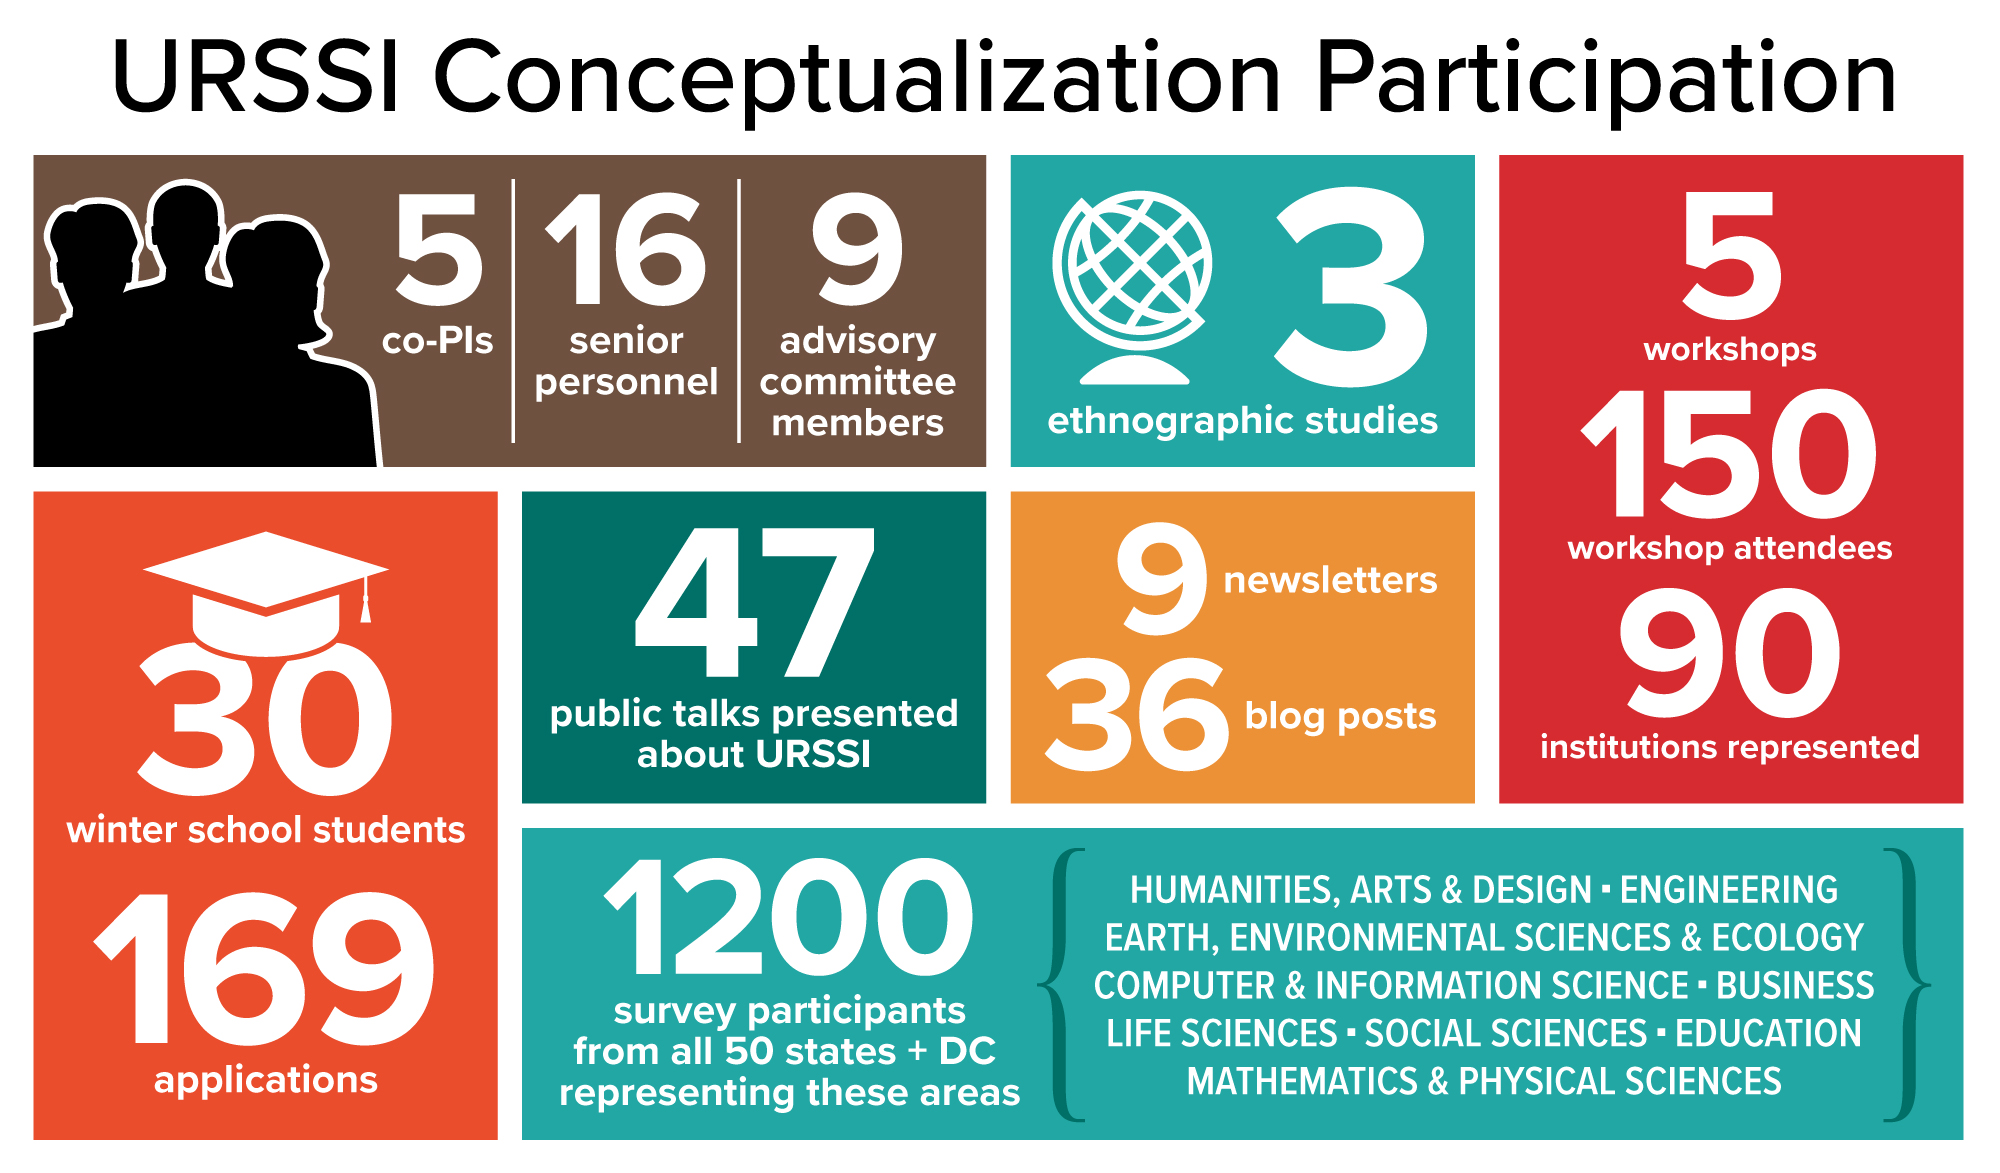
\includegraphics{images/conceptualization_activities.jpg}

\hypertarget{workshops}{%
\section{Workshops}\label{workshops}}

\textbf{Community wide workshops}: In 2018 we held two community workshops with
URSSI stakeholders in Berkeley (April) and Chicago (October). We invited participants
based on their ability to represent diverse roles, institutions, and
perspectives on research software. The general goal of the two community workshops
was to determine which topics this diverse group of stakeholders consider to be
well-understood, which topics still have uncertainty or a need for guidance, and what work
remains to be done in supporting sustainable research software. URSSI PIs
facilitated broad discussions and participated in small group breakout
discussions. Additionally, participants at each workshop gave presentations
about their on-going research software activities.

\textbf{Thematic Workshops}: Participants at the first community workshop identified
two topics worthy of more focused discussion and community input.
We organized the following workshops to better understand those topics:

\begin{itemize}
\item
  The \textbf{Metrics, Credit and Citation Workshop}, held in Santa Barbara,
  California in January 2019, focused on reseach software metrics, citation,
  and impact evaluatin. The 23 participants had strong expertise in the
  various workshop themes, including the PIs of the CodeMeta project, Zenodo,
  and software credit initiatives such as SourceCred.
\item
  The \textbf{Research Incubators Workshop}, held in College Park, Maryland
  in February 2019, focused on methods for incubating new and existing research projects.
  The 20 participants had strong expertise in
  research software project development, including program officers from
  various government agencies, open-source research software developers,
  and organizational scholars that have studied research software processes.
\end{itemize}

\textbf{URSSI Design Workshop}: In April 2019 members of the Senior Personnel
and Advisory Committees participated in a workshop in Chicago, IL. PIs
presented preliminary results from our research (ethnographies and survey)
as well as lessons learned from the four previously held URSSI workshops.

\hypertarget{website-newsletter-blog}{%
\section{Website / Newsletter/ Blog}\label{website-newsletter-blog}}

One of the major goals of the conceptualization project was to build awareness
of the need for an institute, publicize our activities, and increase overall community interest.
To achieve this goal, we used a \href{http://urssi.us}{website}, nine \href{http://urssi.us/newsletter/}{newsletters},
36 \href{http://urssi.us/blog/}{blog posts}, and a seires of public talks and webinars given
by the PIs and others. We sent the newsletters to the URSSI email list, which consists
of workshop attendees and other interested members of the community.
We also publicized the newsletter and blog posts via the \href{https://twitter.com/si2urssi/}{URSSI twitter account},
which has over 500 followers.

\hypertarget{survey}{%
\section{Survey}\label{survey}}

We developed and disseminated a survey to compliment workshop participation.
The primary goal of the survey was to gather the opinions, preferences, and
self-reported activities of the research software community regarding
development practices, development tools, training, funding/institutional
support, career paths, credit for software work, and diversity/inclusion.
For each of these topics, we asked a small number of general questions and
then allowed participants to self-select to answer more detailed questions
about any area of particular interest. We distributed the survey to PIs of
currently funded NSF and NIH projects and to relevant mailing lists. The
survey closed in May 2019 after receiving approximately 1200 responses.

The results of the survey highlighted some areas where URSSI could play a
key role in advancing the sustainability of research software in the United States.

\begin{enumerate}
\def\labelenumi{\arabic{enumi}.}
\item
  There was a mismatch between how respondents wanted to allocate their
  time and their actual allocation of time. This result provides an opportunity
  for URSSI to work with developers and teams to help them focus their efforts
  on the tasks that are most relevant.
\item
  The aspects of the software development process respondents viewed as
  being more difficult than they should be tended to be people-related
  activities rather than technical activities. This result suggests that URSSI
  could support teams and developers by providing training and/or
  resources related to human factors in the software development process.
\item
  Respondents indicated they use a number of software development practices.
  However, one key practice that was underutilized is peer code review. URSSI
  can provide training on peer code review and work with teams to ensure that
  the infrastructure is in place to appropriately support this activity in the
  research software space.
\item
  The respondents indicated that software development practices including
  \emph{requirements}, \emph{design}, \emph{maintenance}, and \emph{documentation} were not
  well-supported by tools.
\item
  In terms of version control, there is still a sizable percentage of
  people who use methods like \emph{copying files to another location} and
  \emph{zip file backups} as version control. This result suggests that URSSI
  could provide additional training and tools to help teams use modern
  version control systems.
\item
  Many of the items above relate to training, or the lack thereof. The
  survey results suggest a large percentage of respondents have not received
  training in software development. While the respondents indicated there were
  sufficient opportunities for training, most of them suggested they did not
  have sufficient time for training. URSSI could help by providing training
  in different formats that work better with the demands of the research
  software developers' environments.
\item
  Many respondents also found the level of support, in terms of funding,
  to be inadequate to be successful. URSSI could help by advocating both at
  the national funding level as well as at the University level for increased
  funding for important research software development activities.
\item
  Respondents also indicated their software contributions were not
  significantly valued in performance reviews. URSSI could help by developing
  and advocating for policies that help research software developers get
  adequate recognition for their work.
\item
  Most projects lack a formal diversity plan. URSSI could help by providing
  template diversity plans and support for developing
  appropriate plans for individual projects.
\end{enumerate}

\hypertarget{ethnography}{%
\section{Ethnography}\label{ethnography}}

To gain a deeper understanding of the practices and experiences of researchers
who are actively engaged in software development, we have undertaken a series of
ethnographic studies. These studies focused on software projects of varying
size and complexity in the fields of hydrology, astronomy, and biochemistry.
Using observations, semi-structured interviews, and a
series of archival documents, we produced case studies of how, over time, these
projects overcame challenges of recruiting contributors, building a governance
model, seeking funding, and sharing credit in sustaining a software project that
has demonstrable impact on a community of researchers.

We developed two of these studies, Astropy and Rosetta Commons, as full case
studies. Both projects face unique sustainability challenges that they solved
somewhat differently. While the main findings of this work are not novel
in the sense that they will surprise anyone familiar with challenges to sustaining
research software, the value of this work is in comparing the two cases. By better
understanding common approaches to overcoming sustainability challenges, we believe
there is a valuable opportunity to abstract these approaches into models of success
that research software projects in other domains can modify or tailor.
The following is a brief summary of the findings from these two case studies.

Points of comparison:

\begin{itemize}
\item
  \emph{Distributed work coordination}: Key to the success of both Astropy and Rosetta
  Commons is coordination of remote collaborative work. Astropy mirrors Python's
  core development team in structuring contributor guidelines and supporting
  designated maintainers. Rosetta Commons differs substantially in that the project
  employs four full-time infrastructure maintainers. This offloading of
  maintenance responsibilities frees up contributors (distributed labs throughout
  the USA) to focus on conducting research and driving innovations that extend
  Rosetta's key functionality.
\item
  \emph{Funding}: Astropy is fiscally sponsored by NumFocus, but depends upon grant
  funding from a variety of sources to sustain its collective work. A recent
  grant from Gordon and Betty Moore Foundation, ``Sustaining and Growing the
  Astropy Project,'' is focused exclusively on maintenance and governance for
  the project's long-term viability to practicing astronomers. Rosetta Commons
  combines licensing and grant funding to sustain its work. Licenses for
  commercial use and an NIH infrastructure maintenance grant have continuously
  supported the project since 2005.
\item
  \emph{Credit}: Both projects have had a number of papers published about their
  development. Astropy suggests two publications to cite when acknowledging
  use of the software \citep{robitaille2013astropy, price2018astropy}. These two
  publications, combined, have over 3000 citations. Rosetta Commons,
  because it has many versions, methods, and language specific implementations,
  has no canonical citation. Interviews with contributors to Rosetta noted
  that this lack of canonical citation causes confusion for authors when rushing towards publication.
  Many researchers have sought a centralized source they could acknowledge.
  Despite the lack of a canonical citation, two papers describing Rosetta and
  its use in predicting protein structures have, combined, over 4300
  citations \citep{rohl2004protein, salmena2011cerna}.
\end{itemize}

We observe differences in the two projects that seem marginal at first
glance, but upon further analysis have important practical consequences
for software development activities. For example, two substantial
differences in the projects have consequences for the long-term sustainability
of each project:

\begin{itemize}
\item
  Astropy, in following an open model of contribution, focuses time and
  attention on clearly documenting and making contributor guidelines
  accessible to research software engineers. The maintenance team
  therefore focuses their effort on ensuring contributors are supported
  while simultaneously keeping various packages up to date and available
  to the community that depends upon this code for their research. This approach is
  partially a result of the software ecosystem being broadly useful to a
  discipline (Astronomy), as compared to Rosetta Commons, which focused on
  specific analytic tasks within a subfield of biological engineering
  (Macromolecular modelling).
\item
  Continuous annual grant funding and licensing fees allow Rosetta to
  centralize infrastructure tasks to a core team whose sole job is
  maintenance. This approach in turn encourages innovation and expansion of feature
  sets for labs that focus solely on producing new research insights.
  Astropy has, over time, centralized maintenance of the project's software
  development and maintenance. But until very recently, this maintenance has been a
  volunteer activity. Shifting time, attention, and energy towards organizing
  an open-source model of development impacts career trajectories for
  practicing astronomers and contributes to a more fragile ecosystem for astronomy.
\end{itemize}

We recognize that software sustainability is more than just financial support,
but what these case studies make clear is that the economic realities of
maintaining and contributing to software development have important downstream
impacts that shape innovation and engagement. The URSSI conceptualization
has studied how these challenges can be practically overcome.

\hypertarget{winter-school}{%
\section{Winter School}\label{winter-school}}

In late December 2019 we ran our
first ever URSSI school on research software engineering. We began accepting
applications in July and received an overwhelming response to our call for
applications. For the 30 participant slots available, we received 169
applications, meaning we had a challenging time selecting the participants
and had to turn away a large number of interested researchers. While the
selection committee used multiple criteria to evaluate and select participants,
successful applicants already had some experience with Python programming, Git,
and Unix skills, which was necessary to benefit from the workshop. Our goal
was not to repeat the same material covered in bootcamps and Software Carpentry
style workshops, but to focus on the research software engineering skills that
not formally taught in any setting. These skills include best practices
for packaging code as software, testing, collaborative software development,
code review, and related topics such as licensing and archiving. The school
lasted 2.5 days.

Based on the demand described above, this experience made evident the strong
need for the skills covered in the school. The overall feedback from the
school was also positive (more on that below). Some key lessons from this
pilot that impact our design of a Summer School as part of URSSI are: 1) the
school needs to be longer to allow for both discussion time and focused time
for students to work on their own code, applying the lessons from the lectures;
and 2) the presence of additional helpers outside of the primary instructors was
quite beneficial to help answer specific questions from the students.

A few example quotes from the Winter School feedback form include:

\begin{itemize}
\item
  ``I really can't say enough good things about this super empowering workshop!
  You did an amazing job identifying the things I didn't know that I didn't know,
  and teaching them at a level that was immediately actionable in my work.''
\item
  ``Thank you so much to everyone for taking this amazing initiative to teach young
  scientists on software sustainability.''
\item
  ``Thank you for putting together this winter-school, it was super useful to me
  and I'm looking forward to applying everything I learned to my future projects
  and to go deeper into the topics that were covered.''
\end{itemize}

\hypertarget{joint-activities}{%
\section{Joint Activities}\label{joint-activities}}

During the URSSI conceptualization process, we helped start two new activities that
overlapped our goals, both so that we could promote these goals and also so
that we could build up these future partners of a later full URSSI institute.

\hypertarget{research-software-alliance-resa}{%
\subsection{Research Software Alliance (ReSA)}\label{research-software-alliance-resa}}

URSSI instigated (along with the UK \href{https://software.ac.uk}{Software Sustainability Institute}
and \href{https://ardc.edu.au}{Australian Research Data Commons}) a global community
of organizations interested in promoting and sustaining software, called the
\href{http://www.researchsoft.org}{Research Software Alliance (ReSA)}. ReSA has
held three meetings, at RSE18, eScience2018, and RSEConUK19, with representatives
from about 20 other organizations and has assembled a mailing list with about 40
such organizations and an umbrella organization under which all these groups can
collaborate to strengthen all of our activities. ReSA is currently working on
defining governance and other activities to formalize ReSA, and at the same time,
it has started a set of \href{http://www.researchsoft.org/resa-taskforces-join-us/}{task forces}
to 1) analyze and document the landscape of different communities and topics of
interest for the research software community (e.g., preservation, RSEs, citation,
productivity, sustainability), 2) collect and share evidence for the importance of
research software, and 3) assemble and maintain a register of research software
funding opportunities. Additionally, ReSA is currently working with other members
of the scholarly community to start up a task force to define FAIR for software,
likely co-organized with \href{https://www.force11.org/}{FORCE11} and
\href{https://www.rd-alliance.org/}{RDA}.

\hypertarget{research-software-engineering-rse}{%
\subsection{Research Software Engineering (RSE)}\label{research-software-engineering-rse}}

In a 2012 workshop sponsored by the UK SSI, a number of UK researchers who develop
software realized that while they internally recognized a number of common elements
to the work they did, along with others at their universities, there was no
commonality to how others saw this work and these roles, and they needed to come
together to build and develop a community. As stated by James Hetheringon, they
decided they needed to ``develop the profession of a scientific software engineer
and the career track of software developers in academia.'' They studied academic job
descriptions in the UK, and found about 10000, of which about 400 were related to
software development, with 194 different job titles. To build recognition of the
common software elements of these positions, they chose the name ``research software
engineer''. They then began publicizing this idea, building a community of people who
identified with the role and encouraged them to also identify with this title,
building RSE groups in UK universities, encouraging universities to change their
job titles, holding workshops and then conferences for RSEs, encouraging a funding
agency to provide fellowships to RSEs, and building up an association with about
2000 members, which later developed into a professional society \citep{RSEHettrick}.

As a number of non-UK people (including some URSSI PIs) started attending UK RSE
conferences, the SSI also supported activities to grow the international community.
These self-developed and SSI-supported activities have led to RSE groups in Germany,
the Netherlands, the Nordic countries, the US, Canada, and South Africa, some of
which have now held national workshops and conferences. The US Research Software
Engineer Association (US-RSE) formed in 2018, with the support and participation
of three of the five URSSI PIs, and has 340 members as of February 2020. The US-RSE
Association is centered around three main goals:

\begin{itemize}
\item
  \emph{Community}: to provide a coherent association of those who identify with the role
  (not necessarily title) of Research Software Engineer, and to provide the members
  of the community the ability to share knowledge, professional connections, and resources.
\item
  \emph{Advocacy}: to promote RSEs' impact on research, highlighting the increasingly
  critical and valuable role RSEs serve.
\item
  \emph{Resources}: to provide useful resources to multiple demographics, including technical
  and career development resources, and information and material to support the
  establishment and expansion of RSE positions and groups within the research ecosystem.
\end{itemize}

There are thus some overlaps between US-RSE's goals and URSSI's and a clear reason
for us to work together going forward.

\hypertarget{synthesis-of-urssi-activities}{%
\section{Synthesis of URSSI Activities}\label{synthesis-of-urssi-activities}}

In the following section we describe common challenges and dilemmas we
identified across URSSI's conceptualization activities. Where possible, we identify
the role URSSI could play in helping overcome these challenges as a funded institute.

\textbf{Challenge 1: Decentralized expertise}

Throughout the planning activities, the community of stakeholders recognized
that there already exist a number of individual efforts to help improve the
development, maintenance, and overall sustainability of research software in
the US. While these efforts, collectively, are comprehensive in their scope,
the decentralized structure of this expertise is inefficient for both resource
discovery and delivery of services. For example there are many points of expertise
in research software development (e.g., SWEBOK, RSEs), education and training
(e.g., academic initiatives, Carpentries), credit and metrics (e.g., CitAs),
incubation (e.g., ESIP, the UW eScience Institute) that are available to
individuals at specific institutions. However, there is currently no comprehensive
organization that can serve to coordinate these activities, promote centers of
expertise, and ensure that effort is not duplicated-- a role that is played
admirably in the UK by the Software Sustainability Institute.

As a coordinating center, URSSI could help solve this challenge in the following ways:

\begin{itemize}
\item
  Broker connections between points of expertise and serve to coordinate
  efforts and funding such that different experts could better collaborate on
  sustainable development, education, and policy initiatives.
\item
  Identify and convene experts to help fill gaps that exist between service
  delivery, for example, where the Carpentries see gaps in knowledge skill or
  acquisition in sustaining software education.
\item
  Disseminate best practices from specific disciplines to the broader
  research community. By acting as a center of research software excellence
  URSSI could be a space where solutions from one domain could be learned and
  efficiently transferred to another.
\item
  Coordinate and help to curate relevant research software packages through
  discovery portals, such as \url{https://libraries.io/}
\end{itemize}

\textbf{Challenge 2: Pathways to sustainability for non-commercial research software}

Throughout the URSSI conceptualization activities, participants voiced concern
for the viability of valuable software projects that do not seek
commercialization. Technology transfer programs at universities and through
research funding agencies (e.g.~I-Corps, SBIR/STTR) are well established
and have been successful at helping entrepreneurially-focused software projects
recognize and execute viable business models. This transition pathway is
promoted for software that has a potential to sustain itself through fees or
licensing agreements. However, there is no equivalent university guidance for
software projects that would like to pursue non-commercial open source models
for sustainability.

There is a need for a US-based institute, divorced from any single university,
to help valuable research software projects realize a non-commercial
open-source route to sustainability. This support could include a program, such as an
incubator, that would guide research software projects towards developing
open-source governance, budgeting, licensing, and fiscal sponsorship in service
of non-commercial sustainability. We view this route, and its guidance from an
institute, as critical to promoting an ecosystem of diverse research software
projects that may not be readily amenable to commercialization, or have the
potential to build healthy and viable volunteer developer communities as an
alternative to licensing.

\textbf{Challenge 3: Coordinated advocacy and analysis for policy change}

Related to the first challenge of decentralized expertise, there is a need
for coordination and targeted leadership around policy for sustainable
research software. Participants in URSSI workshops described a need for
coordinating communities around emerging national, institutional, and even
disciplinary specific policies that have a downstream impact on sustainability,
such as software citation principles, tenure and promotion guidelines that
recognize research software contributions, sustained funding or financial
support for research software maintenance, and software management plans
that explicitly document expectations around software development and archiving.

Currently, community members take on many of these policy activities as additional
professional service, or as volunteer work. This secondary focus on any
one policy issue, in turn, leads to slow progress, high turnover of volunteers,
and does not allow any one person or institution to develop the deep expertise
needed for effective sustained analysis or advocacy.

An institute that could dedicate time and attention to policy design, invest
personnel time in developing needed expertise, and coordinate a sustainable
lobbying network would allow advocacy work to become more manageable,
effective, and result in better outcomes for research software stakeholders.
Further, there is often a need to conduct advocacy work driven by
empirical research that can substantiate how or why one policy decision is
better than another. An institute dedicated to these activities would
facilitate data-driven policy research that could lead to stronger advocacy
positions, and benefit funding agencies, universities, and research
institutions that seek to adopt new policy aimed at improving research
software sustainability.

\textbf{Challenge 4: Signals of viability}

A valuable contribution of the URSSI workshop and engagement activities has
been convening stakeholders with expertise in the evaluation and funding of
research software. These stakeholders include current and former program officers
from NSF, NIH, DoE, DoD, and IMLS, as well as philanthropic organizations
like the Gordon and Betty Moore and Alfred P. Sloan foundations. These
participants have a collective desire for an institute to develop stronger
signals of a research software project's viability; to help evaluate a
project's potential for long-term sustainability; and help communities of
research software stakeholders coalesce around strategic funding initiatives
that could benefit research through software investments.

A dedicated US institute focused on software sustainability could help meet
this challenge in a number of ways, but we recognize that there is no
overarching or simple solution. The plan we describe below explains,
in numerous places, how URSSI can and should convene different communities
to address complex problems like strategic financial investment, evaluation
for viability, etc.

\textbf{Challenge 5: Career Advancement and Credit}

Closely related to Challenges 1, 3 and 4 is a desire of URSSI stakeholders to
see an institute dedicate time and resources towards promoting recognition
for research software activities and helping to shape reliable career pathways
for research software engineers (RSEs). At URSSI workshops, there was
near-unanimous agreement that the acknowledgement of research software
contributions remains difficult for career advancement and there is a lack
of clear guidance for both universities and funding agencies on how to make
progress on these issues.

A dedicated US-based institute for research software sustainability could
play a leading role in advocating for best practices in the measurement,
reward, and credit for research software activities. This activity would include
dedicated research into measuring and evaluating software development activities,
advancing techniques for use and user impact evaluation, and promoting formative
metrics that are conducive to long-term viability. Relatedly, a dedicated US-based
institute could better evaluate and promote the impact of research software
engineering positions that currently exist and advocate for their creation
where they do not.

In the next chapter, we describe URSSI's plan to meet each of these challenges.
In particular, we focus on how a strategic investment in a US-based software
sustainability institute would practically organize itself, allocate budgets,
and measure progress on each of the challenges identified in the conceptualization phase.

\hypertarget{chapter3}{%
\chapter{URSSI Plan}\label{chapter3}}

Throughout the URSSI conceptualization process, the team worked on overall
planning iteratively, using slides at workshops and the URSSI website to
disseminate current thoughts, using the survey and the ethnographic studies as
inputs, using workshops (including slides and shared note documents) and the
discuss forum (\url{https://discuss.urssi.us}) to gather and record feedback. Together,
these activities plus internal discussions of the team and a focused mission and
vision working group have led to most of the content of this document.

\hypertarget{mission-and-vision}{%
\section{Mission and Vision}\label{mission-and-vision}}

URSSI PIs began to develop mission and vision statements in late 2018. The intent
of these statements was to succinctly state the purpose for URSSI's existence
(mission) and based on that purpose what URSSI strives to achieve (vision). The
process for developing these statements was:

\begin{itemize}
\item
  At the first two workshops, we asked participants about the goals and vision
  that a US research software sustainability institute should pursue.
\item
  The URSSI PIs then identified institutions with similar goals and collected
  their mission and vision statements for comparison.
\item
  Eight members of the Senior Personnel and Advisory Committee participated in
  a working group focused on developing URSSI's mission and vision statement.
\item
  Each working group participant provided a written set of three mission and
  three vision statements based on the conceptualization proposal, workshop
  participant's feedback, and guidance from the URSSI PIs.
\item
  Neil Chue Hong, director of the Software Sustainability Institute in the UK,
  facilitated a synthesis of the working group's feedback. This synthesis process included a
  teleconference with participants to discuss and refine versions of each
  mission and vision statement.
\item
  The URSSI PIs then presented drafts of each statement to workshop participants
  at the final URSSI meeting in Chicago and refined a final version of each statement.
\end{itemize}

The mission and vision of URSSI are as follows:

\textbf{Mission}: Our mission is to improve the recognition, development, and use of
software for a more sustainable research enterprise. We achieve this mission
through collaboratively developing education, outreach, and software services
that emphasize open, transparent reproducible, and cooperative practices. URSSI
is an institute for software expertise as well as a social infrastructure that
promotes an inclusive and diverse community of research software engineers,
maintainers, contributors, and users.

\textbf{Vision}: Empowered people, building better software, enabling exceptional research

\hypertarget{planning-assumptions-methods-and-principles}{%
\section{Planning assumptions, methods, and principles}\label{planning-assumptions-methods-and-principles}}

The following assumptions are inputs to our planning process:

\begin{itemize}
\item
  We will propose an institute with a 5-year duration and a potential 5-year
  extension, based on NSF's current institutes and published documents.
\item
  The budget of URSSI will be \$3m-\$5m per year. We take \$3m as the baseline
  minimum funding level needed to operate an institute, below which an institute
  is not the right method to achieve the mission and vision, and then build higher
  cost and higher return activities on that baseline.
\item
  There is demonstrated interest in supporting some URSSI goals from private
  foundations and potential interest from other federal agencies, so URSSI
  activities should be planned as a set of reinforcing (but separable) activities,
  potentially on different timelines.
\item
  There is a strong need for improved software sustainability across all fields,
  and URSSI cannot solve this need in all fields by itself.
\item
  There are many partners who can help URSSI achieve some of its goals, as there
  is overlap between these goals and the goals of those partners.
\item
  It is not practical for URSSI to directly work with the US software development
  community due to the small size of URSSI and the large size of the community, so
  URSSI needs to work indirectly by leveraging other groups.
\end{itemize}

Given the mission and vision, and our assumptions, we plan to use a set of methods
to ensure that URSSI is successful:

\begin{itemize}
\item
  URSSI must choose a set of initial targeted communities and efforts, focus on
  them for some period, then move on to the next set of targets
\item
  URSSI must work closely with partners to amplify its efforts
\item
  URSSI must be clever about using resources, attempting to achieve multiple outputs
  for activities whenever possible.
\end{itemize}

Guiding principles:

\begin{itemize}
\item
  Leverage existing organizations for authority, credibility, resources
\item
  Focus on individuals (i.e., aim at people not projects)
\item
  Leverage available resources (software, services, credit systems, training
  materials, etc.) where possible rather than reinvent
\item
  Respect and learn from volunteers
\item
  Activities should have an end or a sustainability plan beyond URSSI
\item
  Distinguish between quality (badging/intrinsic) and impact (reuse) measures
\item
  Sustain software by sustaining its communities (stewards, developers, maintainers,
  leaders, active users)
\item
  Coordinate activities rather than start new ones when possible
\item
  Advocate and promote a diversity of career paths, recognizing that no one
  correct version of a career is likely to exist across institutions
\end{itemize}

Some topics are partially or completely out-of-scope for URSSI:
{[}\textbf{TODO}: what should be out-of-scope for URSSI?{]}

\textbf{Software Commercialization}. As an institute, URSSI will position
itself as a broker to existing bodies of knowledge or expertise, and
seek to fill needed gaps where no expertise already exists. Relevant
to this positioning is a route to sustainability through the
commercialization of research software. We view this path to sustainability
as already well supported by existing programs and initiatives, some of
which are already funded by NSF. As a principle, URSSI is not opposed
to or discouraging of research software commercialization. We will actively
seek to learn from and collaborate with the commercial software ecosystem,
including technology transfer offices that provide structured pathways to
commercialization for research software in academic institutions. In this
role, URSSI might guide people in deciding if commercialization is a
realistic or good choice for their software project, and connect those who
decide that it is to existing support programs like
\href{https://www.nsf.gov/news/special_reports/i-corps/}{I-Corps}. What we believe
URSSI can uniquely provide, and what we find to be lacking, is support for
alternative routes to sustainability through open-source or non-commercial
fiscal sponsorship. While these alternative routes are obviously less
straightforward, and more challenging they remain the most viable option for
improving the long-term accessibility and impact of most research
investments in software. A majority of even the best research software projects
won't be commercially viable given the size and scope of their audience. It is
this critical gap, between commercialization and open-source, that URSSI seeks
to close.

\hypertarget{desired-impact}{%
\section{Desired impact}\label{desired-impact}}

URSSI's ultimate desired impact, as stated in the vision, is on scholarly
research in science, engineering, and the humanities. URSSI aims to achieve
this impact by contributing resources and training to the research software
ecosystem that will improve research software and to empower the people who
create and maintain that software

For software, URSSI aims to improve the sustainability of research software by

\begin{itemize}
\item
  Developing and sharing good-enough and best practices for software projects,
  including for testing, governance, codes of conduct, continuous integration
\item
  Documenting sustainability models and providing guidance on how to choose among them
\item
  Promoting communities and appropriate governance models for open source research software
\item
  Building models to make best use of and support transient software contributors (e.g.~students)
\end{itemize}

For people, URSSI aims to improve the careers of those who develop and maintain
research software by:

\begin{itemize}
\item
  Promoting new career paths for those who develop and maintain research software
\item
  Developing and advocating for research software usage and impact metrics to be
  a factor in the hiring and promotion of software developers and maintainers
\item
  Promoting the publication of research software
\item
  Creating and providing training for those who want to develop and maintain
  research software
\item
  Encouraging a diverse set of participants to enter the research software
  development and maintenance field and decreasing structural and systemic
  barriers to productive careers for members of underrepresented groups
\end{itemize}

For the research software ecosystem, URSSI aims to improve the understanding and functioning of the ecosystem by

\begin{itemize}
\item
  Documenting the use of research software in research and providing
  systematic and regular analysis of the impact this software has on research
\item
  Growing and participating in communities around the field of research software
\item
  Promoting an increased understanding of the importance of research software in research
\item
  Promoting software credit and citation mechanisms
\item
  Studying methods to catalog and promote research software
\item
  Supporting the use of software in reproducibility
\end{itemize}

\hypertarget{organization-management}{%
\chapter{Organization \& Management}\label{organization-management}}

Coming soon.

\hypertarget{policy}{%
\chapter{Policy}\label{policy}}

The Policy area's intent is to support the people who develop and maintain research software, and to
support research about research software, to ultimately increase the science \& research impact of
software. It does this by focusing on potential initiatives (actions, mandates, incentives, directives)
decision makers can take to have a broad influence on the area, sometimes thought of as leverage points,
including strategies and decisions to invest. Policy happens at multiple levels, including national,
funding agency, institution, and research group.

The Policy area's activities are divided into two parts, research and advocacy. Research is the collecting
and analyzing of data, while advocacy is the dissemination of the research results in such a way that it
changes practices.

\hypertarget{subgoals}{%
\section{Subgoals}\label{subgoals}}

The changes that the policy area seeks to make include:

\begin{enumerate}
\def\labelenumi{\arabic{enumi}.}
\item
  In funding agencies, direct funding of software maintenance other software sustainability activities
  is a core part of the mission, e.g., at NSF, this includes all program officers across all directorates
\item
  In universities and academic fields, positions for people developing and maintaining research software
  are available, recognized, and rewarded
\item
  In publishing, support and recognition for software as a core part of science is the norm
\item
  In industry, sharing best practices, coordinating efforts, and contributing to open source software
  projects is the norm
\item
  Open source software is recognized as a key element of open science and reproducibility
\item
  Diversity of software project contributors is Increased
\end{enumerate}

\hypertarget{area-structure}{%
\section{Area Structure}\label{area-structure}}

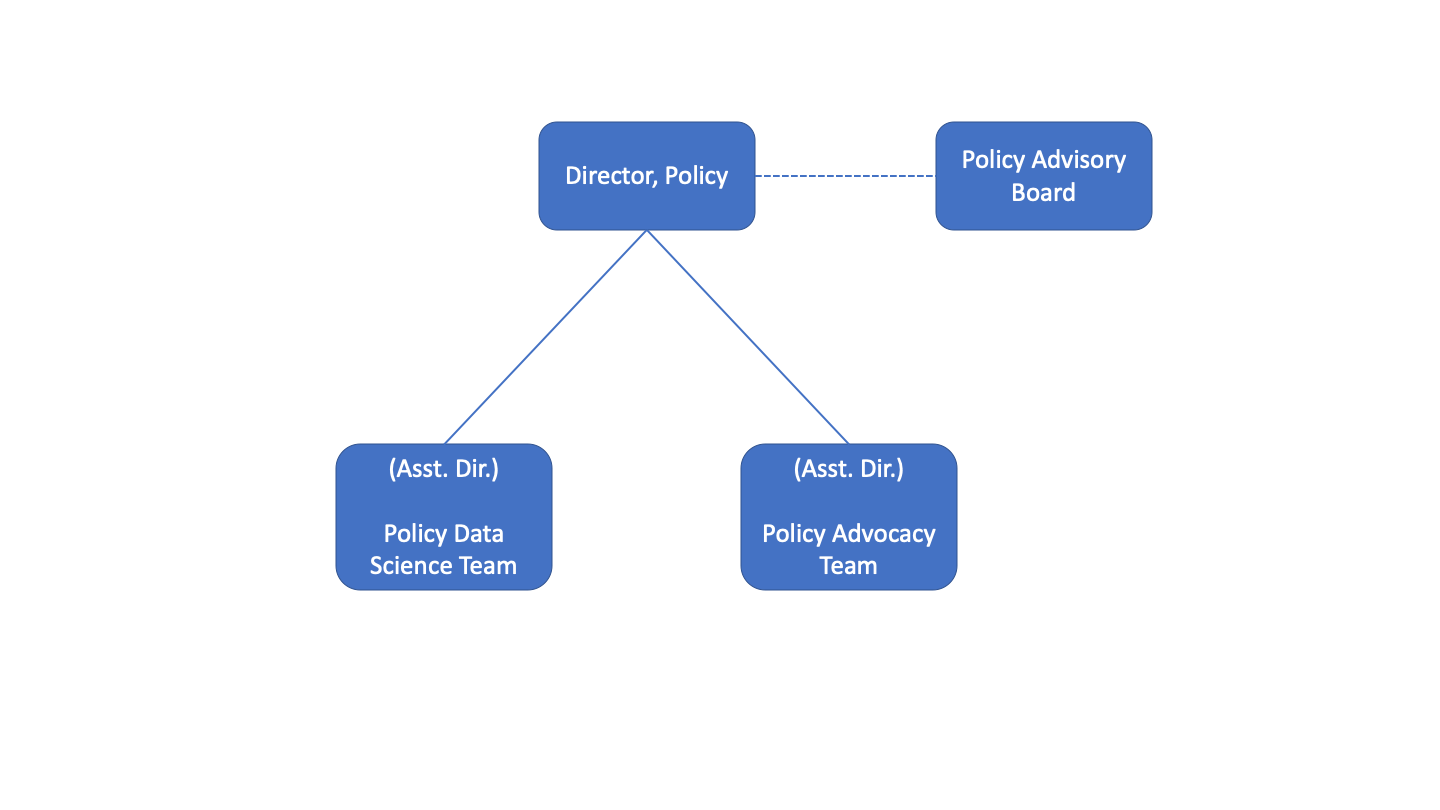
\includegraphics{images/policy_structure.png}

The policy area comprises:

\begin{itemize}
\item
  Director for Policy, an URSSI co-PI, leads the overall Policy area, working with the
  Policy Advisory Board and Policy staff to define and execute policy research and advocacy activities.
\item
  Policy Data Science Team: performs research aimed at informing policy, but not about policy
  itself, for example, with regard to software usage metrics, empirical studies would be most effective.
  Includes funded staff, URSSI fellows, and community volunteers.
\item
  Assistant Director for Policy Advocacy, focuses more on planning advocacy that in doing it,
  by understanding different stakeholders, and building a roadmap for how to effectively advocate
  (within universities, foundations, industry, national labs, etc.)
\item
  Policy Advocacy Team, focused on policy development (such as use cases and examples of practices
  that are effective for sustainability), which ultimately would be used for presenting turnkey ways
  to support research software to institutions, possibly integrating and building upon the data science
  team's findings. Includes funded staff, URSSI fellows, and community volunteers.
\item
  Policy advisory board (appointed volunteers) who provide advice on potential policy area and activities
\end{itemize}

\hypertarget{resources}{%
\section{Resources}\label{resources}}

The policy area will require resources that include funding for salaries, for events, and for travel.

\textbf{Funding for personnel} (e.g., buying out parts of contracts):

\begin{itemize}
\tightlist
\item
  3 FTEs, divided across Assistant Director for Policy Advocacy, Policy Data Science Team
  (potentially a postdoc), Policy Advocacy Team
\end{itemize}

Additional team members, not funded by the policy area:

\begin{itemize}
\tightlist
\item
  Director for Policy, an URSSI co-PI, funded by URSSI at top level
\item
  Policy Advisory Group (appointed volunteers)
\item
  URSSI fellows, working in Policy Data Science Team and Policy Advocacy Team

  \begin{itemize}
  \tightlist
  \item
    (\textbf{TODO}: Fellows program to be run by URSSI Community area; these policy fellows might
    be funded by policy area if needed)
  \end{itemize}
\item
  Other community volunteers, in Policy Data Science Team and Policy Advocacy Team
\end{itemize}

\textbf{Funding for workshops}: \textbf{TODO}: TBD

\begin{itemize}
\tightlist
\item
  Potentially including a policy conference / workshop(s) akin to Aspen Institute / CODATA - \$370k,
  also could be part of an annual URSSI event
\end{itemize}

\textbf{Funding for travel/speaking}: \textbf{TODO}: TBD

If there is less budget available, we would cut back on workshop funding

If there is less budget available, we would:

\begin{itemize}
\item
  Expand policy program to have a summer program for undergraduate and graduate students focused
  on software / science policy (e.g., an REU or something like a google summer of code for policy / law students)
\item
  Hire communication staff to do outreach and engagement around policy topics (would be dedicated
  expertise in policy as opposed to general outreach)
\end{itemize}

\hypertarget{methods-and-processes}{%
\section{Methods and processes}\label{methods-and-processes}}

Initial activities are planned with respect to the set of challenges that follows, but other
challenges can also be introduced. The URSSI leadership group will regularly review suggestions
of new challenges, and will determine a rough desired level of activity across the challenges.

The policy team will then develop and scope activities to match these desired levels, with review
from the Policy Advisory Board, which will also be able to suggest adding or removing challenges
back to the leadership group.

The policy team will also maintain this listing of active, planned, and potential activities and
its mapping to the challenges. Activities will be split into those that, if successful, are likely
to lead to significant changes in 1-2 years, 3-5 years, and longer-term, with an initial goal of
applying 50\% of resources to the 1-2 year activities, 40\% to the 3-5 year activities, and 10\% to
the longer-term activities.

\hypertarget{challenges}{%
\subsection{Challenges}\label{challenges}}

Initially, the policy area has the following set of challenges to address:

\begin{enumerate}
\def\labelenumi{\arabic{enumi}.}
\item
  Career paths (including titles and evaluation criteria for hiring and promotion) aren't well
  established.
\item
  It's hard to measure the impact of individuals, especially in activities that are inherently
  collaborative like software development.
\item
  The academic credit model disincentivizes individual contributions to public goods / infrastructure
\item
  We conflate quality and impact of software and need to disentangle them.
\item
  There is a lack of recognition of the value and importance of software.
\item
  There is a lack of funding opportunities and stable funding for maintenance of software that
  is important but doesn't have a generic market, and ``lumpy'' project funding (projects that are
  competitively funded for fixed periods, often with gaps between funded project periods) means
  that maintenance/sustainability can't be reliably folded into project costs.
\item
  The development and maintenance community is much less diverse than the overall US population.
\end{enumerate}

\hypertarget{partners}{%
\subsection{Partners}\label{partners}}

The Policy area will work with other NSF SI2/CSSI Institutes \& Centers of Excellence
(e.g.~\href{https://sciencegateways.org}{SGCI}, \href{https://molssi.org}{MolSSI}, \href{https://iris-hep.org}{IRIS-HEP}),
the \href{https://www.researchsoft.org}{Research Software Alliance},
the \href{https://software.ac.uk}{Software Sustainability Institute},
the \href{https://us-rse.org}{US-RSE Association},
the (UK) \href{https://society-rse.org}{RSE Society},
The \href{https://www.academicdatascience.org}{Academic Data Science Alliance},
\href{https://carcc.org}{CaRCC},
and any other projects and organizations that also seek to address overlapping challenges.

The Policy area needs to build relationships with the following groups and organizations, and
to work closely with them, particularly in policy activities.

\begin{itemize}
\item
  Institutional and research leaders in the academic and national laboratory community, such as
  VCRs, CTOs/CIOs, who can help URSSI penetrate various institutions and disciplines
\item
  Representatives from professional academic associations
\item
  Representatives from industry (including those already invested and sold on OSS, as well as
  those skeptically interested)
\item
  Representatives from Open Source communities, particularly those that are already effective and working at scale
\item
  People working in science policy, such as in AAAS and the National Academies
\item
  Representatives from organizations and companies serving OSS and RSE communities
  (e.g.~\href{https://numfocus.org}{NumFOCUS}, \href{https://codeforscience.org}{Code for Science \& Society}, GitHub, Code Ocean)
\item
  Representatives from organizations that represent other research support roles
  (e.g., librarians, data stewards, RSEs), to work together to promote all such roles
\item
  Representatives from organizations that focus on diversity and inclusion in academia,
  to encourage them to include software-focused roles where possible
\item
  People from the European Commission regarding European Open Science Cloud (EOSC), etc.
\item
  Representatives from organizations like the Research Data Alliance and FORCE11
\end{itemize}

\hypertarget{planned-activity-pool}{%
\subsection{Planned Activity Pool}\label{planned-activity-pool}}

This is the initial list of activities that URSSI will maintain, and choose from. The specific
activities that will be chosen to start depend on the funding level for URSSI. Most activities
include an amount of effort that is needed to accomplish them. Note that some activities include
raising additional funds for those activities - that fund raising is part of the activity. Other
activities, in the next subsection, are tracked but are beyond the scope of URSSI, and are more
likely activities that others might perform, potentially in coordination with URSSI.

High-level activities include:

\begin{itemize}
\item
  Maintaining the list of potential activities and prioritizing them, including getting inputs
  from the overall community. These inputs will be collected and recorded by all members of the
  project in their interactions with the community, as well as by community members, via tagged
  GitHub issues. Community members will be able to see this list and react with a +1 to issues
  they think are important, and URSSI will use these reactions as an element of prioritization. (ongoing)
\item
  Tracking completed activities and their consequences (ongoing)
\item
  Collecting examples of good and bad policy, structures, and interventions from industry and
  from other disciplines (potential fellow project)
\item
  Developing an advocacy roadmap for how to effectively advocate (to universities, foundations,
  industry, national labs) (policy person \& advisory committee, spread over 3 months)
\end{itemize}

\hypertarget{policy-research-activities}{%
\subsubsection{Policy Research Activities:}\label{policy-research-activities}}

These activities involve research, such as gathering and analyzing evidence and data.

Faculty career path policy - research actions:

\begin{itemize}
\tightlist
\item
  Study tenure guidance and policies, and find/document ways that software work is measured
  and recognized. Publish examples of successes. (2 months)
\end{itemize}

Staff career path policy - research actions:

\begin{itemize}
\item
  Document existing (known successful/viable, known failures) career paths for individuals
  creating research software (2 months)
\item
  Examine and document Industry career paths vs lab career paths vs academic career paths (1 month)
\item
  Create and maintain a mailing list for those interested in career paths (mailing list to be
  supported by Community area) (ongoing, low level of effort)
\item
  Create a clearinghouse of job descriptions with criteria for performance assessment; distill
  out design patterns or different categories for different roles. This could also include documenting
  salary levels for different job descriptions, and connecting the job descriptions with then learning
  modules necessary for these jobs (3-4 months, plus ongoing maintenance)
\item
  Examine how salaries for RSEs compare with those of other researchers? (needs to follow clearinghouse, 1 month)
\end{itemize}

Measuring the impact of individuals policy - research actions:

\begin{itemize}
\tightlist
\item
  Identify factors (manual, such as evaluations, and automated, such as crawling repos) that are
  part of impact and publicize them. Some known factors to investigate include quantifying code
  contributions, code review, mentoring. Determine good practices (for formatting or housing the
  information on these factors) so those factors are discoverable and/or queryable. (6 months)
\end{itemize}

Incentivize contributions to public software policy - research actions:

\begin{itemize}
\item
  Gather data/examples that show when contributions to public projects increase your citation
  count or regular metrics (1 month)
\item
  Gather examples of successful use of individual contributions to public goods/infrastructure
  to gain academic promotion (1 month over 3-6 months)
\item
  Use regular surveys to better understand why people do and don't contribute; get data to
  understand the value of public goods to community (1 month over 3-6 months each year)
\item
  Determine a way to make it easy for scientific communities to peer-review public good software
  (or contributions to such software), with the idea that peer-review is considered a mark of
  quality (ongoing, not well-scoped)
\item
  Research to counter the idea that publishing in the small set of ``highest impact'' journals is
  key, and expose actual impact of work instead (work with scholcom community, use what they have
  done, maybe adapt their work for software - maybe 2 months to start)
\end{itemize}

Disentangle quality and impact of software policy - research actions:

\begin{itemize}
\tightlist
\item
  Create checklists/review guidelines for different levels of peer-review for software; can be
  tiered, could issue stars or use another rating system; leverage information already available
  from journals and other resources. (1 week)
\end{itemize}

Recognize the value and importance of software policy - research actions:

\begin{itemize}
\item
  Find science/discovery cases where software was particularly fundamental, particularly digging
  into software that is not so generally well-known (1 month over 3 months)
\item
  Perform case studies in sustainable software value, e.g., NetCDF, HDF5, DS9 image viewer, GCM
  model(s) --- how much money was invested in these, and how much maintains them? (3-month fellow project)
\item
  Quantify the money that has implicitly funded maintenance and sustainability, and has been saved
  or lost in the shift to open source (e.g., where have funds been spent on one-off software rather
  than maintaining existing open source software, and where has an investment in software maintenance
  saved funds from being spent on one-off software) (3-month fellow project)
\item
  Calculate bus factor for a bunch of key software in disciplines (partner with CHAOSS, or perhaps
  3-month fellow project)
\item
  Document maintenance and funding for critical packages for several disciplines, e.g.~IRAF in astronomy
  (3-month fellow project)
\end{itemize}

Funding opportunities for software maintenance policy - research actions:

\begin{itemize}
\item
  Review the landscape of funding opportunities for software maintenance (and gather data about them)
  and provide a public summary, then keep the summary up-to-date. (jointly done with ReSA? Or CZI EOSS?)
  (1 month and some ongoing work)
\item
  Gather case studies of successful commercialization of open source projects and encourage the
  research community to understand and make use of them (2 months)
\item
  Review the scope of maintenance needs by various research disciplines. Determine the order of
  magnitude of the maintenance backlog for research software (with CHAOSS and others, unscoped)
\end{itemize}

Diversity and inclusion policy - research actions:

\begin{itemize}
\item
  Survey US research software projects to examine diversity of leadership and contributors (3 months)
\item
  Study/survey contributors who make a single contribution and those who make ongoing contributions
  vs membership in underrepresented groups (3 months)
\item
  Contribute to DISCOVER event cookbook{]}(\url{https://discover-cookbook.numfocus.org}), working with
  NumFOCUS's \href{https://numfocus.org/programs/diversity-inclusion}{DISC}
\item
  Other items with CS\&S and NumFOCUS's \href{https://numfocus.org/programs/diversity-inclusion}{DISC},
  for example, creating a cookbook aimed at projects
\end{itemize}

\hypertarget{policy-advocacy-activities}{%
\subsubsection{Policy Advocacy Activities:}\label{policy-advocacy-activities}}

These activities focus on advocacy. They generally depend on policy research or previously
gathered evidence and data.

General advocacy actions (not mapped to specific goals):

\begin{itemize}
\item
  Work with REU programs? -- set up a network of software-focused REUs? Or focus on software
  aspects of more REUs? (provide training, guidance, language for proposals, \ldots)
  (2 month to start + ongoing)
\item
  Play universities (and their administrations) against each other (as has been done by
  the SSI in the UK to create RSE groups), foster competition, by highlighting software work
  (including internal investments to sustain projects that the university sees as important
  and prestigious) and successes (incl funded projects that focus on software) in some universities.
  Rank universities by something and publicize? (maybe with US-RSE) -- via newsletter, blogs,
  press releases (run by URSSI community area? Would accept info from community, e.g.
  Laura Noren's and Brad Stenger's Data Science Community Newsletter (also work with ReSA
  to bi-directionally share info when appropriate)
\item
  Work in citation and credit (get publishers to recognize and highlight software in
  research) (with FORCE11 and others) (minor support of other activities)
\item
  Promote software management plans and software sustainability plans as part of proposals
  (3 months over a year, bringing together community and volunteers, work with ReSA and RDA)
\item
  Develop a set of options for how institutions can support research software (e.g., RSE groups,
  RSE careers, tenure and promotion guidelines) and disseminate it (with US-RSE, starting after year 1)
\item
  Create and operate a professional award program (working with other established organizations)
  e.g., ESA URSSI software award. The URSSI software contribution to research awards: URSSI/ESA
  (e.g.~John Chambers software award from stats association). \$10k funding available from URSSI
  (eventually domain societies would be asked to partially fund the awards). URSSI would need to
  define the categories, criteria/heuristics, etc. for awards beforehand. And find people
  (either staff or community volunteers) to run awards processes (accept nominations, make decisions)
  (2 weeks/year starting in year 2)
\item
  Work with NumFOCUS to provide guidance to projects on how to work with (including obtaining
  funding from) industry (sharing material with incubator area)
\item
  Offer training for software development proposals (or point to others who do)

  \begin{itemize}
  \item
    Develop and disseminate best practices for software development proposals (with NumFOCUS or
    the Capentries)
  \item
    Training/materials could be asynchronous, or in-person with NSF program officers as well, if
    they were willing to do so
  \end{itemize}
\item
  Licensing (in partnership with OSI, Creative Commons, others)

  \begin{itemize}
  \tightlist
  \item
    Provide (pointers to) guidance on licenses and copyright for research software (little work,
    partner with OSI and point to existing best practices)
  \end{itemize}
\end{itemize}

Faculty career path policy - advocacy actions:

\begin{itemize}
\item
  Promote best practices in recognizing and measuring software work in hiring practices and
  tenure letters via sample guidance documents for committees, for faculty, and for
  letter-of-reference authors. (needs focused workshop and follow-through, \textasciitilde3 months over a year)
\item
  Commission a NAS report (similar to the one on \href{https://www.nap.edu/read/25217/chapter/1}{Open Source Software Policy Options for NASA
  Earth and Space Sciences}) on career pathways/progression
  in academia (for scope see last item in next set of bullets)
\end{itemize}

Staff career path policy - advocacy actions:

\begin{itemize}
\item
  Seed ``chapters'' of research software folks (perhaps called URSSI chapters?) at existing
  universities / societies / organizations; create handbook, tools, best practices to support
  local organizers; assign an URSSI ``coordinator'' / community manager. These chapters could:
  talk about training, do consulting for problems, host hacky hours, study groups, software days,
  come together into a larger conference, perhaps an URSSI-wide event. Overall, this
  helps / grows / establishes the community (and make connections that could help chapter members
  meet the right person for their next career moves).

  \begin{itemize}
  \tightlist
  \item
    (TODO: done with URSSI Community area; Policy part (1 month) is creating some materials,
    e.g., guidance on how to set up a chapter, how to align it to local activities, and how to run it.)
  \end{itemize}
\item
  Work to promote and support the establishment of RSE capabilities at universities around the US.
  Provide advice on how to talk to university administrators (and which ones) about this, etc. (1 month,
  jointly with US-RSE)
\item
  Provide examples of language to universities they can use in HR/job ads for RSE positions
  (1 month, jointly with US-RSE)
\item
  Commission a NAS report (similar to the one on \href{https://www.nap.edu/read/25217/chapter/1}{Open Source Software Policy Options for NASA
  Earth and Space Sciences}) on
  \{career pathways/progression in academia, recognition of software, evaluation of software developers,
  inclusion of software in hiring and promotion\} Would need to define, then raise funds from
  outside URSSI (\textasciitilde\$1m), then work with NAS to define a charge and to contract for the study.
  (4 months over 2.5 years)
\end{itemize}

Measuring the impact of individuals policy - advocacy actions:

\begin{itemize}
\item
  Create champions (e.g.~librarians) to promote and educate individuals and projects of these
  good practices (working with Community area) \textbf{TODO}: ref best practices section in Communities
\item
  Help individuals understand how they can best promote themselves (e.g., claim software works on
  ORCID). \textbf{TODO}: ref best practices section in Communities
\end{itemize}

Incentivize contributions to public software policy - advocacy actions:

\begin{itemize}
\item
  Work to persuade high-profile individuals to make public contributions to public projects
\item
  Share examples of successful use of individual contributions to public goods/infrastructure
  to gain academic promotion, produce templates, advocacy toolkits and examples to help others
  to make their case. Similarly, work to persuade people that contributing to projects will
  increase their products within their normally accepted reward system (e.g., get more collaborators
  and papers; increase opportunities to meet/work with new/old collaborators; will build social
  connections/network)
\item
  Show how you can participate in public goods / infrastructure projects (e.g., how to
  structure an issue, how to write your first PR)
  \textbf{TODO}: ref best practices section in Communities
\item
  Produce templates based on successful use of individual contributions to public
  goods/infrastructure to gain academic promotion, advocacy toolkits, and examples to help
  others to make their case (1 month)
\item
  Reframe contributions as first class research products / objects (i.e., explain how building
  the best software is itself science, as it's both discovery and creation). In order to do this,
  amplify existing efforts to build a taxonomy of such contributions to make it clear what those
  contributions are, and encourage people to claim/talk about/take pride in these contributions;
  work with publishers to highlight these contributions and the people who make them. Also advocate
  (materials, webinars, ambassadors, etc.) within academic communities (deans, faculty, science
  societies, review panels, funders) that public software contributions are research (also could
  be done by cross-disciplinary respected groups, such as the national academies)
\item
  Work to revise funder policies to ensure reviewers prioritize grant proposals that reuse,
  build-upon and contribute back to maintenance of public infrastructure
\item
  Create high-profile equivalent of ``highest impact'' journal for software and data work - need
  to reject a lot of work and move it to ``lower class'' venues
\end{itemize}

Recognize the value and importance of software policy - advocacy actions:

\begin{itemize}
\item
  Publicize science/discovery cases where software was particularly fundamental, focusing on
  demonstrating impact of software (1 week/year, ongoing)
\item
  Raise awareness that software needs to be maintained (low level, ongoing)
\end{itemize}

Funding opportunities for software maintenance policy - advocacy actions:

\begin{itemize}
\item
  Encourage funding agencies to require software management/maintenance plans (SMPs).
  Use them to couple the idea of maintenance to the idea of development, to make it clear
  that just doing development without maintenance doesn't work. Note that this leads to
  questions about when maintenance should be stopped, and it's also unclear how long-term
  maintenance would be supported (since grants are by definition time-limited).
  (1-2 months/year ongoing, work with ReSA)
\item
  Advocate for funding agencies to provide a funding pool for short-term maintenance grants
  for existing projects (e.g.~CZI's EOSS program). (1-2 months/year)
\item
  Advocate for universities to support maintenance of software developed by their university
  as part of research impact (or possibly technology transfer). (2 months/year over multiple years)
\item
  Encourage companies to provide funds and channel these funds into maintaining research
  software projects, perhaps via a review process with reviewers from both academic software
  projects and the companies. This could be done jointly with NumFOCUS or a similar organization,
  similar to Tidelift (1-2 months/year)
\end{itemize}

Diversity and inclusion - advocacy actions:

\begin{itemize}
\item
  Advertise \href{https://discover-cookbook.numfocus.org}{DISCOVER event cookbook}, working with
  NumFOCUS's \href{https://numfocus.org/programs/diversity-inclusion}{DISC}
\item
  Other items with CS\&S and NumFOCUS's \href{https://numfocus.org/programs/diversity-inclusion}{DISC},
  such as advertising the cookbook aimed at projects
\item
  Reach out to projects to encourage them to mentor \href{https://www.outreachy.org}{Outreachy} interns
  and those from other programs (e.g.,
  \href{https://www.linuxfoundation.org/about/diversity-inclusiveness/programs/}{Linux Foundation diversity programs},
  \url{https://opensourcediversity.org/\#programs}), and to work with Google Summer of Code, maybe
  include some matchmaking. Consider URSSI as an organization that applies to a set of these
  programs on behalf of a set of software projects.
\item
  Build community mentoring program focused on diversity
\item
  Work with RLadies, Women in Data Science, etc.
\end{itemize}

\hypertarget{unplanned-activity-pool}{%
\subsubsection{Unplanned Activity Pool}\label{unplanned-activity-pool}}

The activities listed here are those that would support URSSI but are beyond the scope of URSSI.
They are listed here to provide ideas to others, and URSSI would potentially be willing to encourage
and support them, but likely without resources.

Staff career path policy - research actions:

\begin{itemize}
\tightlist
\item
  Comparative study of research success at universities with core RSE groups vs those without.
  (potential research topic, not to be started by URSSI)
\end{itemize}

Disentangle quality and impact of software policy - research actions:

\begin{itemize}
\item
  Define what software quality means.
\item
  Define what software impact means and how to measure it. Impact can be looked at in many
  ways: scientific, economic, societal, etc.
\item
  Define how you know what software will be impactful (signals of high impact)
\item
  Capture the difference between quality and impact in written resources (blog post, paper, etc.)
\item
  Conduct a Delphi study or multiple Delphi studies across or between disciplines to determine
  a consensus on key indicators of software impact and related questions, such as: Does improving
  the quality of software improve its impact?
\item
  Perform randomized experiments of software impact where the treatment is improved software practices
\item
  Perform a retrospective study of software quality as related to ``impact'' of that software.
\end{itemize}

Recognize the value and importance of software policy - research actions:

\begin{itemize}
\tightlist
\item
  Study whether higher-quality software produces higher-impact science or more reliable science results
\end{itemize}

General advocacy actions

\begin{itemize}
\tightlist
\item
  Talk about problems with current software licenses/models and suggest alternatives
\end{itemize}

Incentivize contributions to public software policy - advocacy actions:

\begin{itemize}
\tightlist
\item
  Run a help desk once a week on-line for people who are running into difficulties in making contributions and need help
\end{itemize}

Funding opportunities for software maintenance policy - advocacy actions:

\begin{itemize}
\item
  Provide a system to match open source maintenance needs and open source programmers
  (e.g., classified ads), to be funded by URSSI, or URSSI could support proposals for such
  maintenance work (both morally and by providing guidance to the proposer)
\item
  Provide fellowships for programmers to ``do good stuff'' related to maintenance
\item
  Attach money for maintenance to some of the to-be-created awards for good software
  development, jointly named and funded with other communities
\end{itemize}

\hypertarget{work-with-other-parts-of-urssi}{%
\section{Work with other parts of URSSI}\label{work-with-other-parts-of-urssi}}

\begin{itemize}
\item
  Training -- use to learn about problems, use training events to disseminate products and advocacy
\item
  Community -- provide topics for fellows, work with on newsletter and dissemination, host champions,
  contribute to and disseminate best practices
\item
  Incubator -- develop both general and specific guidance for projects
\end{itemize}

\hypertarget{metricsmilestones}{%
\section{Metrics/Milestones}\label{metricsmilestones}}

\begin{itemize}
\item
  Amount of funding provided by US public and private funding agencies for research software
  development and maintenance
\item
  Number of US universities with RSE-like positions
\item
  Number of US university faculty who successfully use software work as an important part of
  their tenure packages
\item
  \textbf{TODO}: more needed
\end{itemize}

\hypertarget{education-training}{%
\chapter{Education \& Training}\label{education-training}}

Coming soon.

\hypertarget{incubator}{%
\chapter{Incubator}\label{incubator}}

Coming soon.

\hypertarget{community-outreach}{%
\chapter{Community \& Outreach}\label{community-outreach}}

Coming soon.

\hypertarget{final-words}{%
\chapter{Final Words}\label{final-words}}

We have finished a nice book.

  \bibliography{references.bib}

\end{document}
